
\documentclass[11pt,a4paper]{article}

\usepackage[utf8]{inputenc}
\usepackage[T1]{fontenc}
\usepackage[spanish]{babel}

\usepackage{tgpagella}
\usepackage{geometry}
\usepackage{graphicx}
\usepackage{xcolor}
\usepackage{titlesec}
\usepackage{fancyhdr}
\usepackage[parfill]{parskip}
\usepackage[expansion=false]{microtype}
\usepackage{hyperref}
\usepackage{setspace}
\usepackage{needspace}

\geometry{top=3.0cm,bottom=3.0cm,left=3.5cm,right=3.5cm}

\setlength{\parskip}{0.65em}
\setlength{\parindent}{0em}

\definecolor{azulai}{RGB}{30,80,140}
\definecolor{doradoai}{RGB}{140,90,0}
\definecolor{grisai}{RGB}{70,70,70}

\titleformat{\section}
{\Large\bfseries\color{azulai}}
{}{0em}{}
[{\color{azulai}\titlerule[0.5pt]}]

\titlespacing*{\section}{0pt}{1.8em}{0.8em}

\titleformat{\subsection}
{\large\bfseries\color{doradoai}}
{}{0em}{}

\titlespacing*{\subsection}{0pt}{1.2em}{0.4em}

\pagestyle{fancy}
\fancyhf{}

\rhead{\textcolor{grisai}{\small Maite Barragan — Arquitectura Interna}}
\lhead{\textcolor{grisai}{\small Carta Natal Base}}

\cfoot{\textcolor{grisai}{\small\thepage}}

\renewcommand{\headrulewidth}{0.3pt}

\hypersetup{
colorlinks=true,
linkcolor=azulai,
urlcolor=azulai
}

\setstretch{1.4}

\begin{document}

% ── PORTADA ──────────────────────────────────────────────────────────────

\begin{titlepage}

\centering

\vspace*{1.5cm}

{\Huge\bfseries\color{azulai} Carta Natal Base}\\[0.5cm]

{\large\color{grisai} Arquitectura Interna}\\[0.4cm]

{\small\itshape\color{grisai}
Un método para sostener cuerpo, energía y vida con coherencia
}\\[2cm]

{\huge\color{doradoai} Maite Barragan}\\[1.5cm]

{\Large 07/01/1971 \quad 12:15}\\[0.3cm]

{\Large Pamplona, España}\\[0.3cm]

{\normalsize
Lat: 42.8157° \quad
Lon: -1.6522° \quad
UTC+01:00
}\\[0.5cm]

{\normalsize
Ascendente: Aries 6°18'
}\\[2.5cm]

\vfill

{\small Generado el 20/05/2026}

\end{titlepage}


% ── INTRODUCCIÓN ─────────────────────────────────────────────────────────────

\section*{Introducción}

Esta carta natal base no busca definir quién eres.

La astrología se utiliza aquí como lenguaje de observación:
una forma de mirar cómo se organiza tu energía,
qué registros aparecen con más facilidad
y qué dinámicas pueden influir en tu manera de vivir, sostenerte y relacionarte con el entorno.

No se trata de una lectura predictiva ni de una identidad fija.
Es un mapa inicial de orientación.

Las siguientes páginas muestran únicamente las capas principales de la carta:
los ejes más visibles,
la distribución general de la energía
y algunos patrones básicos desde los que sueles moverte.

\vspace{0.4cm}

\newpage


% ── RUEDA ────────────────────────────────────────────────────────────────

\section{Carta Natal}

\begin{center}
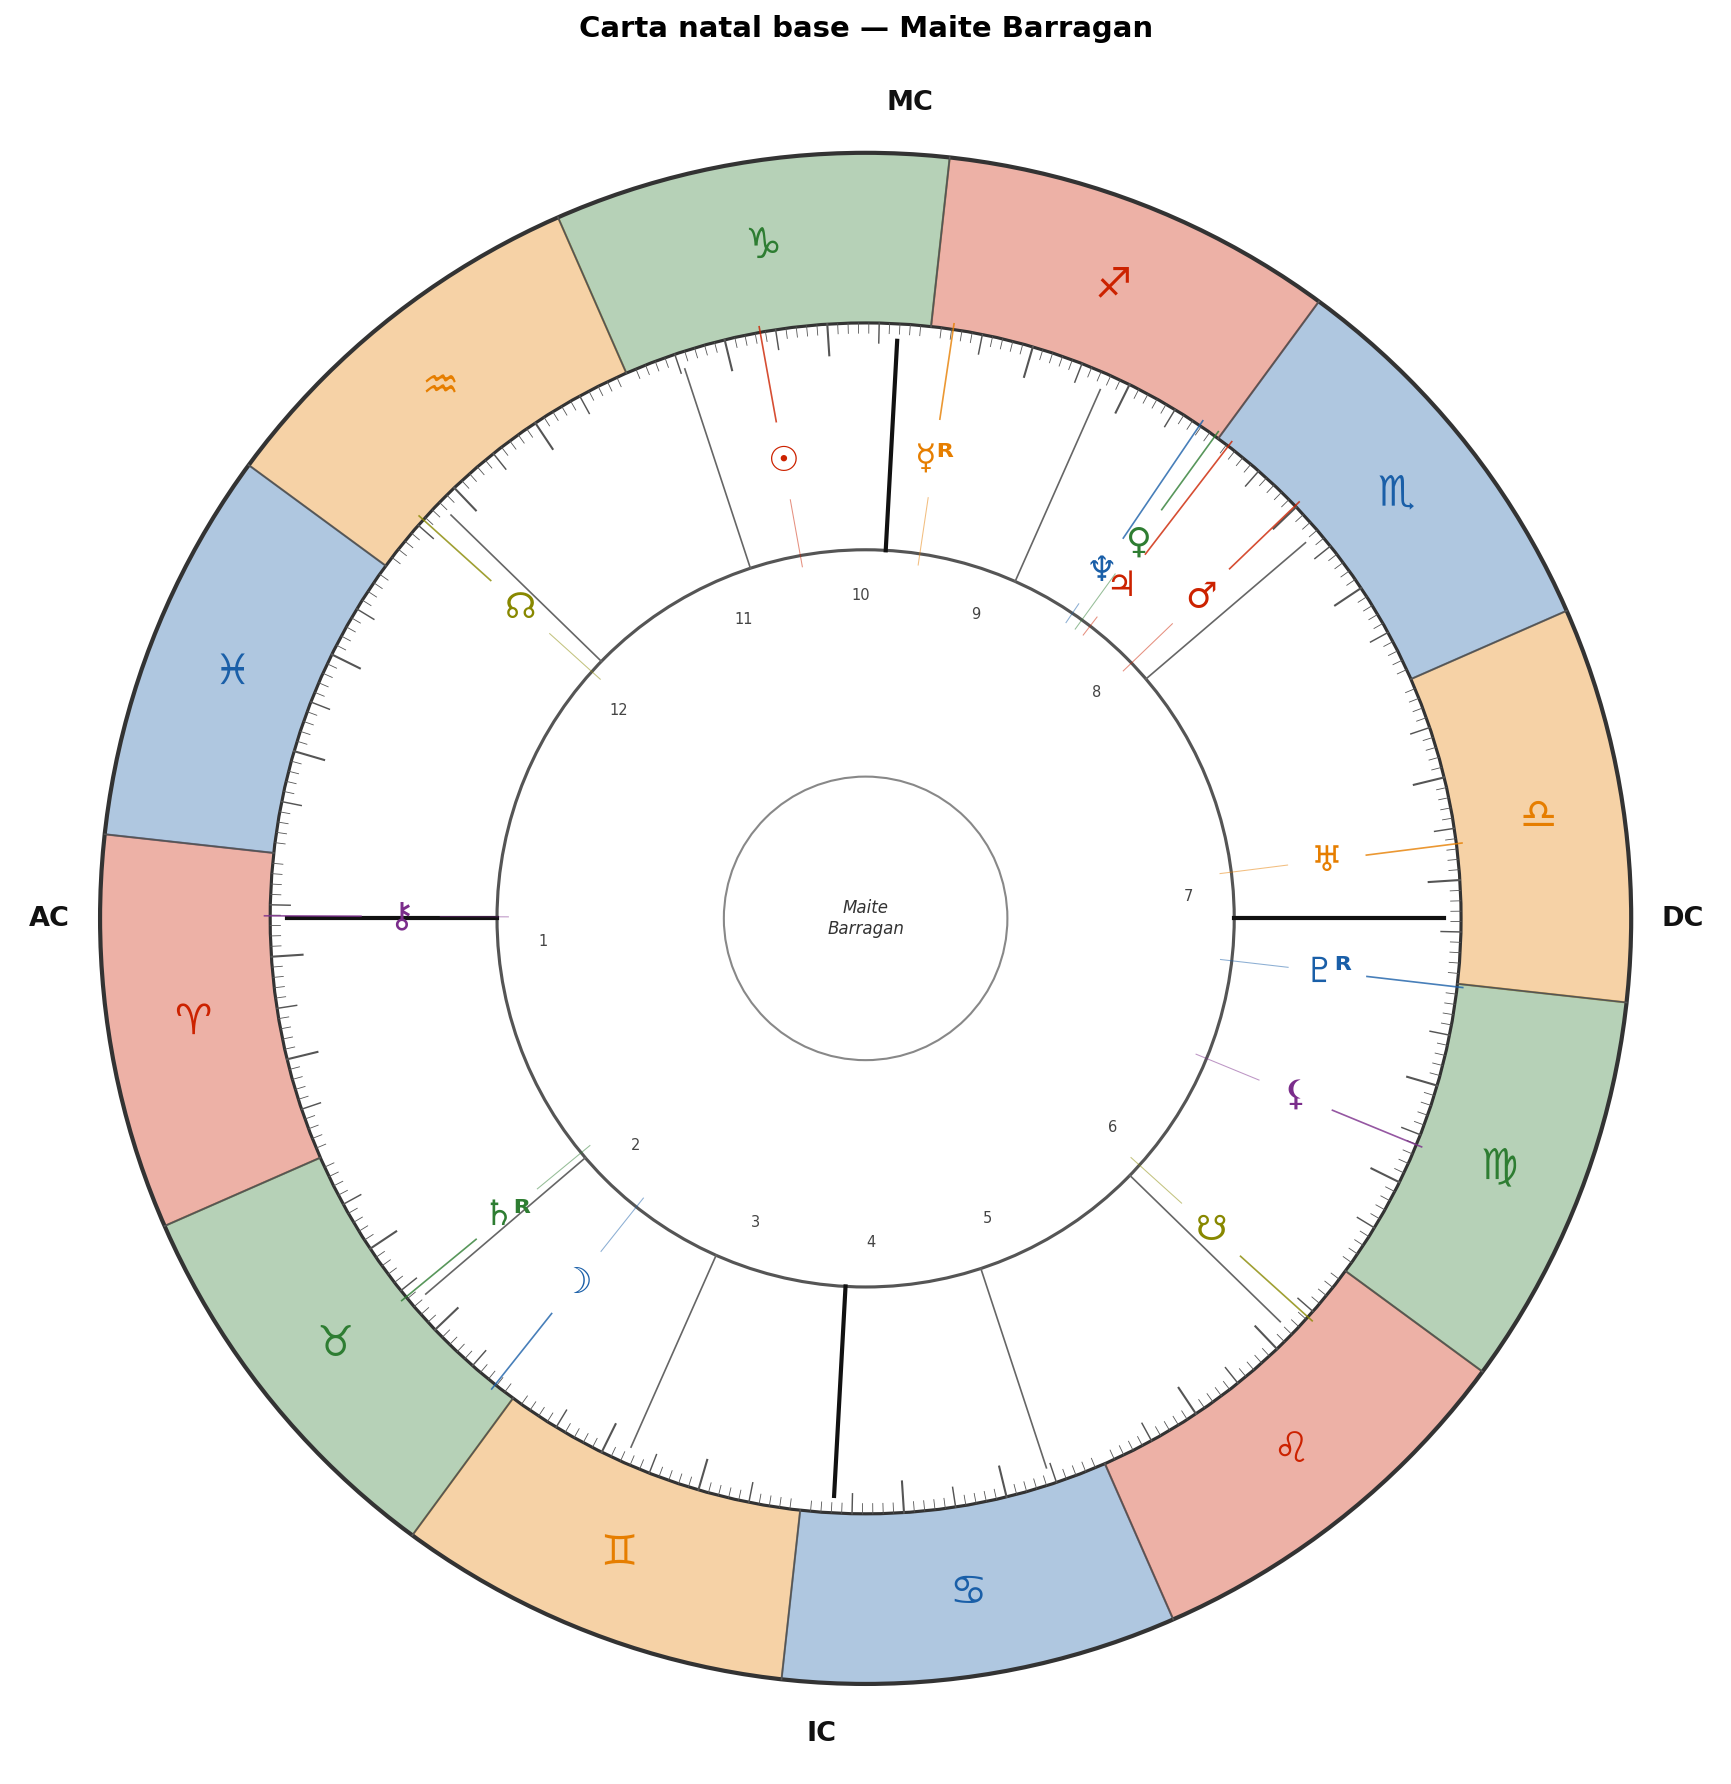
\includegraphics[width=0.8\textwidth]{Maite_Barragan_carta_base_rueda.png}
\end{center}

\vspace{0.8cm}

% ── POSICIONES PRINCIPALES ───────────────────────────────────────────────

\section{Posiciones principales}

\begin{center}

Sol en Capricornio — Casa 10\\
Luna en Tauro — Casa 2\\
Ascendente Aries\\
Medio Cielo en Capricornio

\end{center}

\vspace{0.5cm}

{\small\itshape
La lectura ampliada desarrolla el mapa completo de posiciones,
aspectos y configuraciones de la carta.
}

\vspace{0.8cm}
\Needspace{5\baselineskip}

% ── VISIÓN GENERAL ───────────────────────────────────────────────────────

\section{Visión general}

Tu carta muestra esta distribución de elementos: Fuego 6, Tierra 6, Aire 1, Agua 3.5. El elemento más presente es Fuego (iniciativa, impulso y necesidad de movimiento) y Tierra (estabilidad, concreción y contacto con lo práctico). Esto señala un registro que suele aparecer con facilidad en tu forma de funcionar. El elemento menos presente es Aire (pensamiento, comunicación y necesidad de perspectiva). No significa ausencia, sino una cualidad que puede necesitar más atención consciente. Predomina la modalidad fija, asociada a la constancia, la continuidad y la capacidad de sostener lo importante. Tu Medio Cielo en Capricornio orienta tu presencia pública hacia la responsabilidad, estructura y construcción a largo plazo.

\vspace{0.8cm}
\Needspace{5\baselineskip}

% ── LOS TRES PILARES ────────────────────────────────────────────────────

\section{Los tres pilares}

\subsection{Sol en Capricornio}

Con el Sol en Capricornio, tiendes a construir tu vida de forma gradual, responsable y sostenida. Sueles valorar el esfuerzo, la experiencia y aquello que puede mantenerse de forma sólida en el tiempo. Tu energía puede parecer lenta al principio, pero normalmente gana fuerza con la constancia. Con el Sol en Casa 10, la vocación, el reconocimiento y la construcción de algo visible suelen tener bastante importancia en tu vida. Necesitas sentir que lo que haces tiene coherencia con quién eres y hacia dónde quieres ir. Muchas veces el desarrollo profesional influye directamente en tu sensación de dirección y estabilidad.

\vspace{0.8cm}
\Needspace{5\baselineskip}

\subsection{Luna en Tauro}

Con la Luna en Tauro, normalmente necesitas estabilidad, calma y cierta continuidad emocional para sentirte bien. Las emociones suelen asentarse despacio y no te resulta fácil cambiar rápidamente de estado interno. El contacto con lo conocido, lo sencillo o lo corporal suele ayudarte a recuperar equilibrio. Con la Luna en Casa 2, la estabilidad y la sensación de seguridad suelen influir mucho en cómo te sientes emocionalmente. Los recursos, el cuerpo y aquello que puedes sostener de forma concreta suelen tener bastante importancia para ti.

\vspace{0.8cm}
\Needspace{5\baselineskip}

\subsection{Ascendente Aries}

Con Ascendente en Aries, sueles entrar en los entornos de forma directa, rápida y con bastante iniciativa. Las demás personas normalmente perciben una presencia activa y con energía desde el primer momento. Muchas veces necesitas sentir libertad para actuar a tu manera.

\vspace{0.8cm}
\Needspace{5\baselineskip}

% ── CIERRE ───────────────────────────────────────────────────────────────

\section{Cierre}

Esta carta no busca definirte ni darte una identidad fija.

La astrología se utiliza aquí como lenguaje de observación:
una forma de mirar tendencias, ritmos y maneras de relacionarte con la vida.

La lectura ampliada desarrolla con más profundidad:
los vínculos,
la regulación emocional,
los patrones repetitivos,
la dirección de crecimiento,
las tensiones internas
y las configuraciones principales de la carta.

La lectura completa no busca darte más información.
Busca ayudarte a entender cómo sostener tu vida sin romperte por dentro.

\vspace{1cm}

\begin{center}

{\small\itshape\color{grisai}
Arquitectura Interna
}

\end{center}

\end{document}
